\documentclass[tikz,border=4pt]{standalone}
\begin{document}
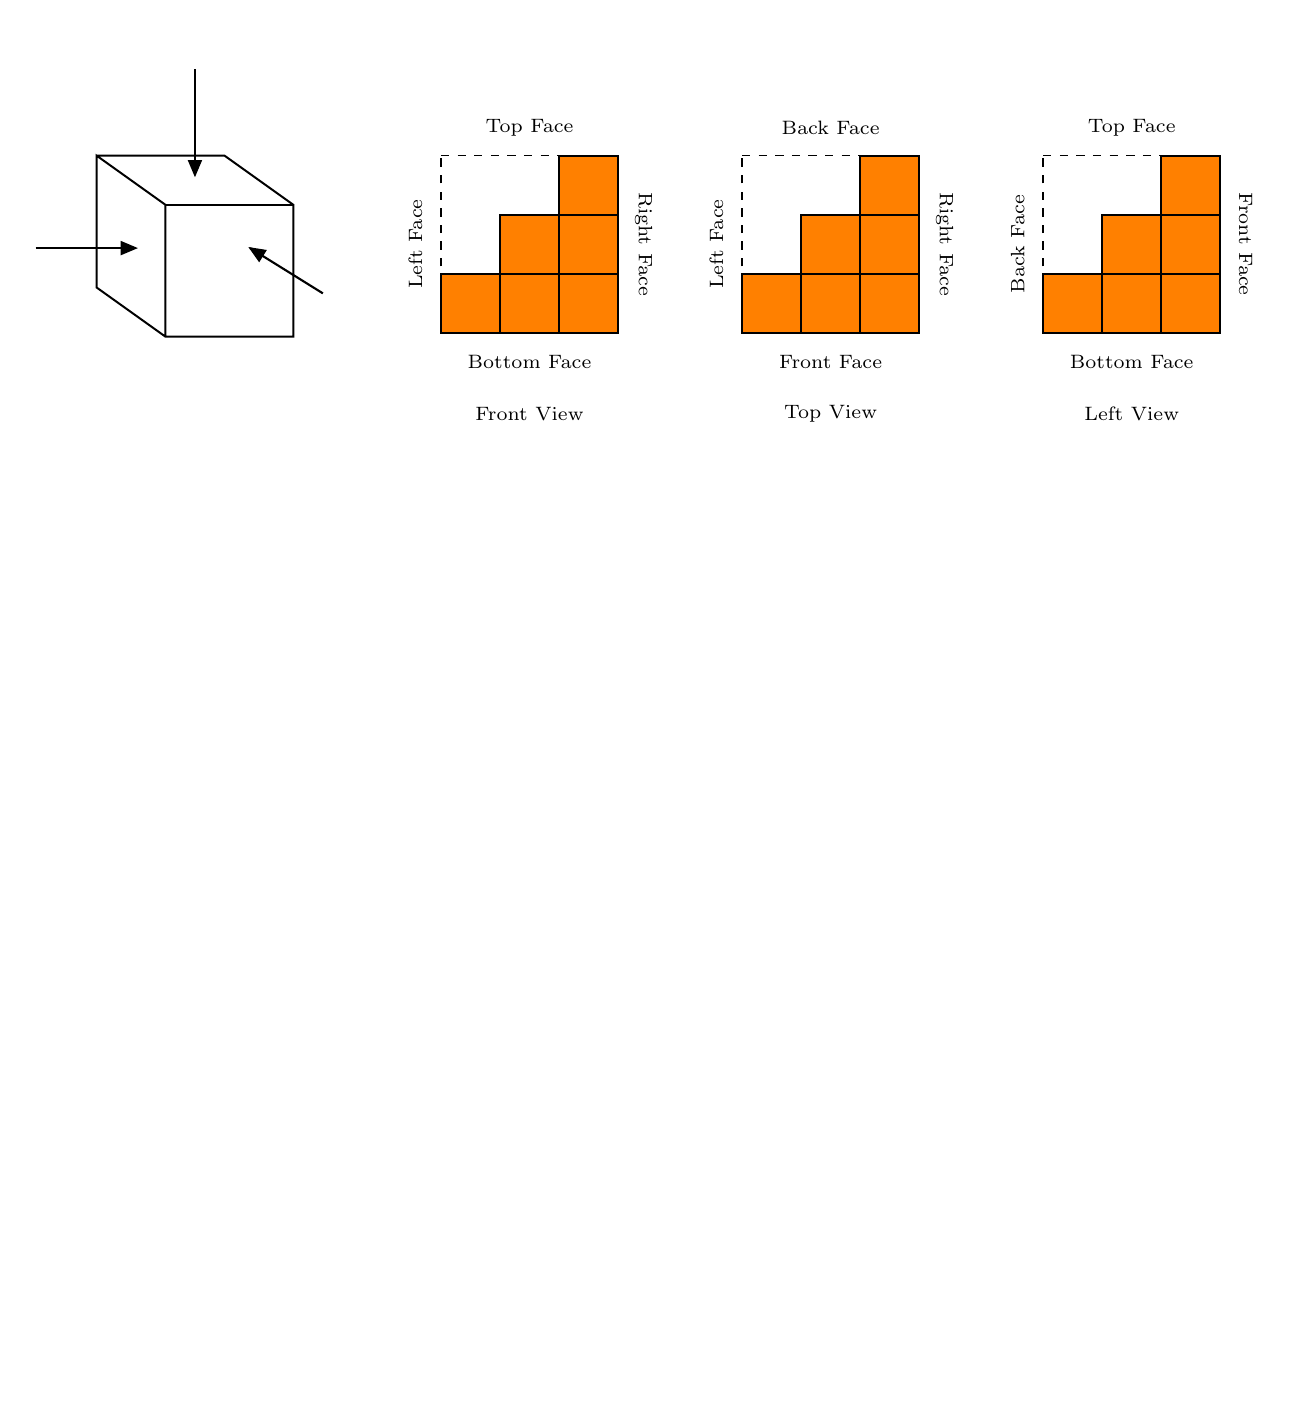
\begin{tikzpicture}[x=.025cm,y=-.025cm]
\path[use as bounding box] (0,0) rectangle (640,690);
\path[draw=black,fill=none,line width=0.7150000000000001pt] (35,65) -- (100,65) -- (135,90) -- (135,157) -- (70,157) -- (35,132) -- (35,65) -- (70,90) -- (70,157);
\path[draw=black,fill=none,line width=0.7150000000000001pt] (70,90) -- (135,90);
\path[draw=black,fill=none,line width=0.77pt] (85,21) -- (85,75);
\path[draw=black,fill=black,line width=0.55pt] (85,75) -- (81.8847,67.6315) -- (88.1153,67.6315) -- cycle;
\path[draw=black,fill=none,line width=0.77pt] (4,112) -- (55,112);
\path[draw=black,fill=black,line width=0.55pt] (55,112) -- (47.6315,115.1153) -- (47.6315,108.8847) -- cycle;
\path[draw=black,fill=none,line width=0.77pt] (150,135) -- (113,112);
\path[draw=black,fill=black,line width=0.55pt] (113,112) -- (120.9026,113.2443) -- (117.6133,118.5359) -- cycle;
\path[draw=black,fill=none,line width=0.55pt,dashed] (210,65) -- (300,65) -- (300,155) -- (210,155) -- cycle;
\path[draw=black,fill=orange,line width=0.7150000000000001pt] (270,65) -- (300,65) -- (300,95) -- (270,95) -- cycle;
\path[draw=black,fill=orange,line width=0.7150000000000001pt] (240,95) -- (270,95) -- (270,125) -- (240,125) -- cycle;
\path[draw=black,fill=orange,line width=0.7150000000000001pt] (270,95) -- (300,95) -- (300,125) -- (270,125) -- cycle;
\path[draw=black,fill=orange,line width=0.7150000000000001pt] (210,125) -- (240,125) -- (240,155) -- (210,155) -- cycle;
\path[draw=black,fill=orange,line width=0.7150000000000001pt] (240,125) -- (270,125) -- (270,155) -- (240,155) -- cycle;
\path[draw=black,fill=orange,line width=0.7150000000000001pt] (270,125) -- (300,125) -- (300,155) -- (270,155) -- cycle;
\node[inner sep=0pt,font=\scriptsize] at (255,51) {Top Face};
\node[inner sep=0pt,font=\scriptsize,rotate=90] at (197,110) {Left Face};
\node[inner sep=0pt,font=\scriptsize,rotate=-90] at (313,110) {Right Face};
\node[inner sep=0pt,font=\scriptsize] at (255,170) {Bottom Face};
\node[inner sep=0pt,font=\scriptsize] at (255,196) {Front View};
\path[draw=black,fill=none,line width=0.55pt,dashed] (363,65) -- (453,65) -- (453,155) -- (363,155) -- cycle;
\path[draw=black,fill=orange,line width=0.7150000000000001pt] (423,65) -- (453,65) -- (453,95) -- (423,95) -- cycle;
\path[draw=black,fill=orange,line width=0.7150000000000001pt] (393,95) -- (423,95) -- (423,125) -- (393,125) -- cycle;
\path[draw=black,fill=orange,line width=0.7150000000000001pt] (423,95) -- (453,95) -- (453,125) -- (423,125) -- cycle;
\path[draw=black,fill=orange,line width=0.7150000000000001pt] (363,125) -- (393,125) -- (393,155) -- (363,155) -- cycle;
\path[draw=black,fill=orange,line width=0.7150000000000001pt] (393,125) -- (423,125) -- (423,155) -- (393,155) -- cycle;
\path[draw=black,fill=orange,line width=0.7150000000000001pt] (423,125) -- (453,125) -- (453,155) -- (423,155) -- cycle;
\node[inner sep=0pt,font=\scriptsize] at (408,51) {Back Face};
\node[inner sep=0pt,font=\scriptsize,rotate=90] at (350,110) {Left Face};
\node[inner sep=0pt,font=\scriptsize,rotate=-90] at (466,110) {Right Face};
\node[inner sep=0pt,font=\scriptsize] at (408,170) {Front Face};
\node[inner sep=0pt,font=\scriptsize] at (408,196) {Top View};
\path[draw=black,fill=none,line width=0.55pt,dashed] (516,65) -- (606,65) -- (606,155) -- (516,155) -- cycle;
\path[draw=black,fill=orange,line width=0.7150000000000001pt] (576,65) -- (606,65) -- (606,95) -- (576,95) -- cycle;
\path[draw=black,fill=orange,line width=0.7150000000000001pt] (546,95) -- (576,95) -- (576,125) -- (546,125) -- cycle;
\path[draw=black,fill=orange,line width=0.7150000000000001pt] (576,95) -- (606,95) -- (606,125) -- (576,125) -- cycle;
\path[draw=black,fill=orange,line width=0.7150000000000001pt] (516,125) -- (546,125) -- (546,155) -- (516,155) -- cycle;
\path[draw=black,fill=orange,line width=0.7150000000000001pt] (546,125) -- (576,125) -- (576,155) -- (546,155) -- cycle;
\path[draw=black,fill=orange,line width=0.7150000000000001pt] (576,125) -- (606,125) -- (606,155) -- (576,155) -- cycle;
\node[inner sep=0pt,font=\scriptsize] at (561,51) {Top Face};
\node[inner sep=0pt,font=\scriptsize,rotate=90] at (503,110) {Back Face};
\node[inner sep=0pt,font=\scriptsize,rotate=-90] at (619,110) {Front Face};
\node[inner sep=0pt,font=\scriptsize] at (561,170) {Bottom Face};
\node[inner sep=0pt,font=\scriptsize] at (561,196) {Left View};
\end{tikzpicture}
\end{document}
